%!TEX program = xelatex
\documentclass[12pt, a4paper]{article}

\usepackage[dvipsnames]{xcolor}

\usepackage{fancyhdr}
\usepackage{extramarks}
\usepackage{amsmath}
\usepackage{empheq}
\usepackage{amsthm}
\usepackage{amsfonts}
\usepackage{tikz}
\usepackage{tikz-3dplot}
\usepackage[plain]{algorithm}
\usepackage{algpseudocode}

\usepackage{ctex}
\usepackage{indentfirst}
\usepackage{wrapfig}
\usepackage{subfigure}
\usepackage{pgfplots}
\usepgfplotslibrary{patchplots}
\usepgfplotslibrary{colormaps}
\usepgfplotslibrary{colorbrewer}
\pgfplotsset{compat=1.18}
\usetikzlibrary{automata,positioning,shapes.geometric,arrows.meta,patterns,calc}
\numberwithin{equation}{section}
\CTEXoptions[today=old]

%
% Basic Document Settings
%

\topmargin=-0.25in
\evensidemargin=0in
\oddsidemargin=0in
\textwidth=6.5in
\textheight=9.2in
\headsep=0.25in

\linespread{1.1}

\pagestyle{fancy}
\lhead{\hmwkAuthorName}
\chead{\hmwkClass : \hmwkTitle}
\rhead{\firstxmark}
\lfoot{\lastxmark}
\cfoot{\thepage}

\renewcommand\headrulewidth{0.4pt}
\renewcommand\footrulewidth{0.4pt}

\setlength{\parindent}{2em}  % 2em代表首行缩进两个字符

%
% Create Problem Sections
%

\newcommand{\enterProblemHeader}[1]{
    \nobreak\extramarks{}{Problem \arabic{#1} continued on next page\ldots}\nobreak{}
    \nobreak\extramarks{Problem \arabic{#1} (continued)}{Problem \arabic{#1} continued on next page\ldots}\nobreak{}
}

\newcommand{\exitProblemHeader}[1]{
    \nobreak\extramarks{Problem \arabic{#1} (continued)}{Problem \arabic{#1} continued on next page\ldots}\nobreak{}
    \stepcounter{#1}
    \nobreak\extramarks{Problem \arabic{#1}}{}\nobreak{}
}

% \setcounter{secnumdepth}{0}
\newcounter{partCounter}
\newcounter{homeworkProblemCounter}
\setcounter{homeworkProblemCounter}{0}
% \nobreak\extramarks{Problem \arabic{homeworkProblemCounter}}{}\nobreak{}

%
% Homework Problem Environment
%
% This environment takes an optional argument. When given, it will adjust the
% problem counter. This is useful for when the problems given for your
% assignment aren't sequential. See the last 3 problems of this template for an
% example.
%
\newenvironment{homeworkProblem}[1][-1]{
    \ifnum#1>0
        \setcounter{homeworkProblemCounter}{#1}
    \fi
    \section{Problem \arabic{homeworkProblemCounter}}
    \setcounter{partCounter}{1}
    \enterProblemHeader{homeworkProblemCounter}
}{
    \exitProblemHeader{homeworkProblemCounter}
}

%
% Homework Details
%   - Title
%   - Due date
%   - Class
%   - Section/Time
%   - Instructor
%   - Author
%

\newcommand{\hmwkTitle}{Vector Algebra and Spatial Geometry}
\newcommand{\hmwkClass}{Advanced Mathematics}
\newcommand{\hmwkClassTime}{}
\newcommand{\myUniversiy}{Wuhan University}
\newcommand{\hmwkAuthorName}{\textbf{Lai Wei}}

%
% Title Page
%

\title{
    \vspace{2in}
    \textmd{\textbf{\hmwkClass:\ \hmwkTitle}}\\
    \vspace{0.4in}
    \large{\textit{\myUniversiy}}
    \vspace{3in}
}

\author{\hmwkAuthorName}
\date{March 2, 2025}

\renewcommand{\part}[1]{\textbf{\large Part \Alph{partCounter}}\stepcounter{partCounter}\\}

%
% Various Helper Commands
%

% Useful for algorithms
\newcommand{\alg}[1]{\textsc{\bfseries \footnotesize #1}}

% % For derivatives
% \newcommand{\deriv}[1]{\frac{\mathrm{d}}{\mathrm{d}x} (#1)}

% For partial derivatives
\newcommand{\pderiv}[2]{\frac{\partial}{\partial #1} (#2)}

% Integral dx
\newcommand{\dx}{\mathrm{d}x}

% Alias for the Solution section header
\newcommand{\solution}{\textbf{\large Solution}}

% Probability commands: Expectation, Variance, Covariance, Bias
\newcommand{\E}{\mathrm{E}}
\newcommand{\Var}{\mathrm{Var}}
\newcommand{\Cov}{\mathrm{Cov}}
\newcommand{\Bias}{\mathrm{Bias}}

% 我的newcommand
\newcommand{\degree}{^{\circ}}
\newcommand{\arrow}{-{Stealth[length=4mm,width=2mm]}}
\newcommand{\rmd}{\mathrm{d}}
\newcommand{\deriv}[2]{\frac{\rmd #1}{\rmd #2}}
\renewcommand{\parallel}{\mathrel{/\mskip-2.5mu/}}
\newcommand{\parallelogram}{
	\mathord
    {\text
        {
			\tikz[baseline]
			\draw (0,.1ex) -- (.8em,.1ex) -- (1em,1.6ex) -- (.2em,1.6ex) -- cycle;
        }
    }
}

\begin{document}

\maketitle

\pagebreak

% 设置页码格式是罗马数字
\pagenumbering{roman}

% 生成目录
\tableofcontents

\pagebreak

% 设置页码格式是阿拉伯数字
\pagenumbering{arabic}

\pagebreak

\section{向量积、混合积}

\subsection{向量积}

\subsubsection{定义}

    设有向量\(\overrightarrow{a}\)、\(\overrightarrow{b}\),其夹角为\(\theta\)。定义新向量,
    记作\(\overrightarrow{a} \times \overrightarrow{b}\),如下:

    \begin{itemize}
        \item 大小:
            \begin{align}
                \lvert \overrightarrow{a} \times \overrightarrow{b} \rvert =
                \lvert \overrightarrow{a} \rvert \cdot \lvert \overrightarrow{b} \rvert \cdot \sin\theta
            \end{align}            
        \item 方向:\(\overrightarrow{a} \times \overrightarrow{b}\)与\(\overrightarrow{a}\)、\(\overrightarrow{b}\)
            都垂直,其指向按右手螺旋定则,由\(\overrightarrow{a}\)沿着不大于\(\mathrm{\pi}\)
            的角度转向\(\overrightarrow{b}\)确定。
    \end{itemize}

\subsubsection{性质}

    \begin{enumerate}
        \item \(\overrightarrow{a} \times \overrightarrow{b} \perp \overrightarrow{a}\),
            \(\overrightarrow{a} \times \overrightarrow{b} \perp \overrightarrow{b}\)
        \item 重要结论:
        \\
        \(\overrightarrow{a} \times \overrightarrow{a} = \overrightarrow{0}\)
        \\
        对非零向量\(\overrightarrow{a}\),\(\overrightarrow{b}\),有\(\overrightarrow{a} \parallel
        \overrightarrow{b} \leftrightarrow \overrightarrow{a} \times \overrightarrow{b} = 
        \overrightarrow{0}\)
        \item 几何意义(向量积的模):
            \begin{equation}
                \begin{aligned}
                    \lvert \overrightarrow{a} \times \overrightarrow{b} \rvert &=
                    \lvert \overrightarrow{a} \rvert \cdot \lvert \overrightarrow{b} \rvert \cdot \sin\theta
                    \\
                    &= S_{\parallelogram}
                \end{aligned}        
            \end{equation}


            \[
                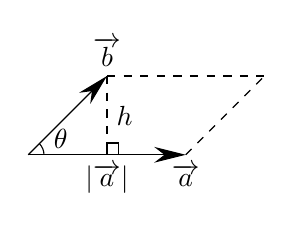
\begin{tikzpicture}
                    \coordinate[label=above:$\overrightarrow{b}$] (b) at (1,1);
                    \coordinate[label=below:$\overrightarrow{a}$] (a) at (2,0);
                    \coordinate[label=right:$\theta$] (theta) at (0.2,0.2);
                    \coordinate[label=right:$h$] (h) at (1,0.5);
                    \coordinate[label=below:$\lvert\overrightarrow{a}\rvert$] (_a_) at (1,0);
                    \draw[\arrow] (0,0) -- (a);
                    \draw[\arrow] (0,0) -- (b);
                    \draw[dashed] (b) -- (3,1);
                    \draw[dashed] (a) -- (3,1);
                    \draw (0.2,0) arc (0:45:0.2);
                    \draw[dashed] (b) -- (_a_);
                    \draw (1,0) rectangle (1.15,0.15);
                \end{tikzpicture}
            \]
            即\(\lvert \overrightarrow{a} \times \overrightarrow{b} \rvert\)表示:
            以\(\overrightarrow{a}\)、\(\overrightarrow{b}\)为邻边的平行四边形的面积。
    \end{enumerate}
    
\subsubsection{运算规律}

    \begin{enumerate}
        \item 反交换律:
            \begin{align}
                \overrightarrow{a} \times \overrightarrow{b} = 
                - \overrightarrow{b} \times \overrightarrow{a}
            \end{align}
        \item 分配律:
            \begin{align}
                \left(\overrightarrow{a} + \overrightarrow{b}\right) \times \overrightarrow{c}
                = \overrightarrow{a} \times \overrightarrow{c} + \overrightarrow{b} \times \overrightarrow{c}
            \end{align}
        \item 结合律:
            \begin{align}
                \left(\lambda \overrightarrow{a}\right) = \lambda \left(\overrightarrow{a}
                \times \overrightarrow{b}\right) = \overrightarrow{a} \times \left(\lambda \overrightarrow{b}\right)
            \end{align}
    \end{enumerate}

\subsubsection{向量积的坐标表示}

    设有向量\(\overrightarrow{a} = \left(x_1, y_1, z_1\right)\)、\(\overrightarrow{b} = \left(x_2, y_2, z_2\right)\),
    则有
    
    \begin{equation}
        \begin{aligned}
            \overrightarrow{a} \times \overrightarrow{b} &= \left(x_1\overrightarrow{i} + y_1\overrightarrow{j}
            + z_1\overrightarrow{k}\right) \times \left(x_2\overrightarrow{i} + y_2\overrightarrow{j} +
            z_2\overrightarrow{k}\right)
            \\
            &= \left(y_1z_2 - z_1y_2\right) \cdot \overrightarrow{i} + \left(z_1x_2 - x_1z_2\right) \cdot \overrightarrow{j}
            + \left(x_1y_2 - y_1x_2\right) \cdot \overrightarrow{k}
            \\
            &= \left(y_1z_2 - z_1y_2,\; z_1x_2 - x_1z_2\,\; x_1y_2 - y_1x_2\right)
            \\
            &= \left|
                \begin{array}{cccc}
                \overrightarrow{i} & \overrightarrow{j} & \overrightarrow{k} \\
                x_1 & y_1 & z_1 \\
                x_2 & y_2 & z_2
                \end{array}
            \right|
        \end{aligned}
    \end{equation}

    同理,

    \[
        \overrightarrow{b} \times \overrightarrow{a} =
        \left|
            \begin{array}{cccc}
            \overrightarrow{i} & \overrightarrow{j} & \overrightarrow{k} \\
            x_2 & y_2 & z_2 \\
            x_1 & y_1 & z_1
            \end{array}
        \right|
    \]

\subsection{混合积}

\subsubsection{定义}

    设有向量\(\overrightarrow{a}\),\(\overrightarrow{b}\),\(\overrightarrow{c}\),称数\(\left(\overrightarrow{a}
    \times \overrightarrow{b}\right) \cdot \overrightarrow{c}\)为向量\(\overrightarrow{a}\),\(\overrightarrow{b}\),
    \(\overrightarrow{c}\)的混合积,记作\(\left[\overrightarrow{a} \; \overrightarrow{b} \;
    \overrightarrow{c}\right]\),即

    \begin{align}
        \left[\overrightarrow{a} \; \overrightarrow{b} \; \overrightarrow{c}\right] =
        \left(\overrightarrow{a} \times \overrightarrow{b}\right) \cdot \overrightarrow{c}
    \end{align}

\subsubsection{坐标表示}

    设有向量\(\overrightarrow{a} = \left(x_1, y_1, z_1\right)\)、\(\overrightarrow{b} = \left(x_2, y_2, z_2\right)\)、
    \(\overrightarrow{c} = \left(x_3, y_3, z_3\right)\),则有

    \begin{align}
        \left[\overrightarrow{a} \; \overrightarrow{b} \; \overrightarrow{c}\right] =
        \left|
            \begin{array}{cccc}
            x_1 & y_1 & z_1 \\
            x_2 & y_2 & z_2 \\
            x_3 & y_3 & z_3
            \end{array}
        \right|
    \end{align}

\subsubsection{几何意义}

    \(\left|\left[\overrightarrow{a} \; \overrightarrow{b} \; \overrightarrow{c}\right]\right|\)表示以
    \(\overrightarrow{a}\),\(\overrightarrow{b}\),\(\overrightarrow{c}\)为相邻三条棱的平行六面体的体积。
    因此,\(\overrightarrow{a}\),\(\overrightarrow{b}\),\(\overrightarrow{c}\)共线\(\Leftrightarrow
    \left[\overrightarrow{a} \; \overrightarrow{b} \; \overrightarrow{c}\right] = 0\)。

\subsubsection{运算规律}

    \begin{equation}
        \begin{aligned}
            &\left[\overrightarrow{a} \; \overrightarrow{b} \; \overrightarrow{c}\right] =
            \left[\overrightarrow{b} \; \overrightarrow{c} \; \overrightarrow{a}\right] =
            \left[\overrightarrow{c} \; \overrightarrow{a} \; \overrightarrow{b}\right]
            \\
            = &- \left[\overrightarrow{a} \; \overrightarrow{c} \; \overrightarrow{b}\right] =
            - \left[\overrightarrow{c} \; \overrightarrow{b} \; \overrightarrow{a}\right] =
            - \left[\overrightarrow{b} \; \overrightarrow{a} \; \overrightarrow{c}\right]
        \end{aligned}
    \end{equation}

    即按照下图沿同一方向(顺时针或逆时针)旋转的混合积组合的值是相等的。

    \[
        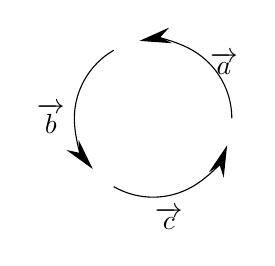
\begin{tikzpicture}
            \coordinate[label=right:$\overrightarrow{a}$] (a) at (0.6,0.7);
            \coordinate[label=left:$\overrightarrow{b}$] (b) at (-1,0);
            \coordinate[label=below:$\overrightarrow{c}$] (c) at (0.2,-1);
            \draw[\arrow] (1,0) arc (0:100:1);
            \draw[\arrow] (-0.5,1.732/2) arc (120:220:1);
            \draw[\arrow] (-0.5,-1.732/2) arc (240:340:1);
        \end{tikzpicture}
    \]

\subsubsection{例题}

    已知\((\overrightarrow{a} \times \overrightarrow{b}) \cdot \overrightarrow{c} = 2\),求\(\left[(\overrightarrow{a} \times \overrightarrow{b}) \times
    (\overrightarrow{b} + \overrightarrow{c})\right] \cdot (\overrightarrow{c} + \overrightarrow{a})\)。

    \textbf{Solution}
    \\


    \[
        \begin{split}
            & \left[(\overrightarrow{a} \times \overrightarrow{b}) \times (\overrightarrow{b} + \overrightarrow{c})\right] \cdot (\overrightarrow{c} + \overrightarrow{a})
            \\
            &= \left[\overrightarrow{a} \times \overrightarrow{b} + \overrightarrow{a} \times \overrightarrow{c} + \overrightarrow{b} \times \overrightarrow{b} +
            \overrightarrow{b} \times \overrightarrow{c}\right] \cdot (\overrightarrow{c} + \overrightarrow{a})
        \end{split}
    \]

    由\(\overrightarrow{b} \times \overrightarrow{b} = 0\),故
    \\

    \[
        \begin{split}
            & \left[(\overrightarrow{a} \times \overrightarrow{b}) \times (\overrightarrow{b} + \overrightarrow{c})\right] \cdot (\overrightarrow{c} + \overrightarrow{a})
            \\
            &= \left[\overrightarrow{a} \times \overrightarrow{b} + \overrightarrow{a} \times \overrightarrow{c} + \overrightarrow{b} \times \overrightarrow{c}\right]
            \cdot (\overrightarrow{c} + \overrightarrow{a})
            \\
            &= \left[\overrightarrow{a} \; \overrightarrow{b} \; \overrightarrow{c}\right] + \left[\overrightarrow{a} \; \overrightarrow{c} \; \overrightarrow{c}\right] + 
            \left[\overrightarrow{b} \; \overrightarrow{c} \; \overrightarrow{c}\right] + \left[\overrightarrow{a} \; \overrightarrow{b} \; \overrightarrow{a}\right] +
            \left[\overrightarrow{a} \; \overrightarrow{c} \; \overrightarrow{a}\right] + \left[\overrightarrow{b} \; \overrightarrow{c} \; \overrightarrow{a}\right]
        \end{split}
    \]

    显然,当混合积中只有不同的两个向量时(可认为这三个向量共面),该混合积值为0。于是

    \[
        \begin{split}
            & \left[(\overrightarrow{a} \times \overrightarrow{b}) \times (\overrightarrow{b} + \overrightarrow{c})\right] \times (\overrightarrow{c} + \overrightarrow{a})
            \\
            &= \left[\overrightarrow{a} \; \overrightarrow{b} \; \overrightarrow{c}\right] + \left[\overrightarrow{b} \; \overrightarrow{c} \; \overrightarrow{a}\right]
        \end{split}
    \]

    由于

    \[
        \left[\overrightarrow{a} \; \overrightarrow{b} \; \overrightarrow{c}\right] =
        \begin{vmatrix}
        a_{x} & a_{y} & a_{z} \\
        b_{x} & b_{y} & b_{z} \\
        c_{x} & c_{y} & c_{z}
        \end{vmatrix}
    \]

    而

    \[
        \left[\overrightarrow{b} \; \overrightarrow{c} \; \overrightarrow{a}\right] =
        \begin{vmatrix}
        b_{x} & b_{y} & b_{z} \\
        c_{x} & c_{y} & c_{z} \\
        a_{x} & a_{y} & a_{z}
        \end{vmatrix}
    \]

    所以

    \[
    \left[\overrightarrow{a} \; \overrightarrow{b} \; \overrightarrow{c}\right] = \left[\overrightarrow{b} \; \overrightarrow{c} \; \overrightarrow{a}\right]
    \]

    于是

    \[
        \begin{split}
            \left[(\overrightarrow{a} \times \overrightarrow{b}) \times (\overrightarrow{b} + \overrightarrow{c})\right] \times (\overrightarrow{c} + \overrightarrow{a})
            = 2 \; \left[\overrightarrow{a} \; \overrightarrow{b} \; \overrightarrow{c}\right]
        \end{split}
    \]

\section{平面及其方程}

\subsection{曲面方程与空间曲线方程的概念}

\subsubsection{曲面方程}

    设有曲面\(S: F\left(x, y, z\right) = 0\),满足

    \begin{enumerate}
        \item 曲面\(S\)上任一点都满足方程;
        \item 不在曲面\(S\)上的点的坐标不满足方程。
    \end{enumerate}

\subsubsection{空间曲线方程}

    设有曲面\(S_1: F_1\left(x, y, z\right) = 0\)和设有曲面\(S_2: F_2\left(x, y, z\right) = 0\),
    联立两方程:

    \[
        \begin{cases}
            F_1\left(x, y, z\right) = 0, \\
            F_2\left(x, y, z\right) = 0.
        \end{cases}
    \]

    满足

    \begin{enumerate}
        \item 曲面\(S\)上任一点都满足方程;
        \item 不在曲面\(S\)上的点的坐标不满足方程。
    \end{enumerate}

\subsection{平面的点法式方程}

    设平面\(\mathit{\Pi}\)上有一点\(M_{0}\left(x_0,y_0,z_0\right)\),其法向量为\(\overrightarrow{n} = \left(
    A, B, C\right)\)。(注意:平面的法向量不唯一。)
    
    设\(M\left(x,y,z\right)\),则\(\overrightarrow{M_{0}M} \perp \overrightarrow{n}\),则
    \(\overrightarrow{M_{0}M} \cdot \overrightarrow{n} = 0\),而\(\overrightarrow{M_{0}M} =
    \left(x-x_0,y-y_0,z-z_0\right)\)。于是
    
    \begin{align}
        A\left(x-x_0\right) + B\left(y-y_0\right) + C\left(z-z_0\right) = 0
        \label{Point-Normal-Plane}
    \end{align}
    
    即为平面\(\mathit{\Pi}\)的点法式方程。

\subsection{平面的一般方程}

    \begin{align}
        Ax + By + Cz + D = 0
        \label{General-Form-Plane}
    \end{align}

    即为平面的一般方程。

    任一三元一次方程的图形总是一个平面,方程\ref{General-Form-Plane}中\(x\)、\(y\)、\(z\)的系数就是该平面的
    一个法向量\(\overrightarrow{n}\)的坐标,即\(\overrightarrow{n} = \left(A, B, C\right)\)。

    特殊情况:

    \begin{enumerate}
        \item \(D=0 \Leftrightarrow \)平面通过原点;
        \item \(A=0 \Leftrightarrow \)平面平行于(或包含)\(x\)轴;
            \\
            \(B=0 \Leftrightarrow \)平面平行于(或包含)\(y\)轴;
            \\
            \(C=0 \Leftrightarrow \)平面平行于(或包含)\(z\)轴;
        \item \(A=B=0 \Leftrightarrow \)平面平行于(或重合于)\(xOy\)平面;
            \\
            \(B=C=0 \Leftrightarrow \)平面平行于(或重合于)\(yOz\)平面;
            \\
            \(A=C=0 \Leftrightarrow \)平面平行于(或重合于)\(xOz\)平面;
        \item \(A=D=0 \Leftrightarrow \)平面包含\(x\)轴;
            \\
            \(B=D=0 \Leftrightarrow \)平面包含\(y\)轴;
            \\
            \(C=D=0 \Leftrightarrow \)平面包含\(z\)轴;
        \item \(A=B=D=0 \Leftrightarrow z=0\)(\(xOy\)平面);
            \\
            \(B=C=D=0 \Leftrightarrow x=0\)(\(yOz\)平面);
            \\
            \(A=C=D=0 \Leftrightarrow y=0\)(\(xOz\)平面);
    \end{enumerate}

\subsection{平面的截距式方程}

    \begin{align}
        \frac{x}{a} + \frac{y}{b} + \frac{z}{c} = 1
        \label{Intercept-Form-Plane}
    \end{align}

    即为平面的截距式方程。方程\ref{Intercept-Form-Plane}中\(a\),\(b\),\(c\)即分别为平面在\(x\),\(y\),\(z\)
    轴上的截距。

\subsection{两平面的夹角}

\subsubsection{定义}

    两平面的法线向量的夹角(通常指锐角或直角)称为两平面的夹角。因此\(\cos \theta = \left|\cos
    \left(\hat{\overrightarrow{n_1}, \overrightarrow{n_2}}\right)\right|\)。

    设平面\(\mathit{\Pi_{1}}\)和\(\mathit{\Pi_{2}}\)的法线向量依次为\(\overrightarrow{n_{1}} = \left(A_{1}, B_{1}, C_{1}\right)\),
    \(\overrightarrow{n_{2}} = \left(A_{2}, B_{2}, C_{2}\right)\)。按两向量夹角的余弦的坐标表示式平面\(\mathit{\Pi_{1}}\)
    和\(\mathit{\Pi_{2}}\)的夹角\(\theta\)可由

    \begin{align}
        \cos \theta=\frac{\left|A_1 A_2+B_1 B_2+C_1 C_2\right|}
        {\sqrt{A_1^2+B_1^2+C_1^2} \sqrt{A_2^2+B_2^2+C_2^2}}
    \end{align}

    来确定。

\subsubsection{结论}

    \begin{enumerate}
        \item \(\mathit{\Pi_{1}}\)和\(\mathit{\Pi_{2}}\)相互垂直相当于\(A_1 A_2+B_1 B_2+C_1 C_2=0\)
        \item \(\mathit{\Pi_{1}}\)和\(\mathit{\Pi_{2}}\)相互平行相当于\(\dfrac{A_1}{A_2}=\dfrac{B_1}{B_2}=\dfrac{C_1}{C_2}\)
    \end{enumerate}

\subsection{点到平面的距离}

    设点\(P_{0}\left(x_0, y_0, z_0\right)\)是平面\(Ax + By + Cz + D = 0\)外一点,则\(P_0\)到该平面的距离为

    \begin{align}
        d=\frac{\left|A x_0+B y_0+C z_0\right|}{\sqrt{A^2+B^2+C^2}}
    \end{align}

    设有两平行平面\(\mathit{\Pi_{1}}: Ax + By +Cz +D_1 = 0\)和\(\mathit{\Pi_{1}}: Ax + By +Cz +D_2 = 0\),则两平面间的距离为

    \begin{align}
        d=\frac{\left|D_1 - D_2\right|}{\sqrt{A^2+B^2+C^2}}
    \end{align}

\section{空间直线及其方程}

\subsection{空间直线的一般方程}

    \begin{equation}
        L:\left\{\begin{array}{l}
        A_1 x+B_1 y+C_1 z+D_1=0 \\
        A_2 x+B_2 y+C_2 z=D_2=0
        \end{array}\right.
    \end{equation}

    注意:空间直线的方程是不唯一的。

\subsection{空间直线的对称式方程}

    \(L\)上有一点\(M_0\left(x_0, y_0, z_0\right)\),非零方向向量\(\overrightarrow{s} =
    \left(m, n, p\right)\),设\(L\)上任一点\(M_0\left(x, y, z\right)\),则
    \(\overrightarrow{M_{0}M} \parallel \overrightarrow{s}\),而\(\overrightarrow{M_{0}M} =
    \left(x-x_0, y-y_0, z-z_0\right)\),所以

    \begin{align}
        \frac{x-x_0}{m}=\frac{y-y}{n}=\frac{z-z_0}{p}
    \end{align}

    即为直线的对称式方程(或称点向式方程)
    
    注意

    \begin{enumerate}
        \item 非零向量\(\overrightarrow{s} = \left(m, n, p\right)\)称为\(L\)的方向向量(不唯一);
        \item 直线上任一方向向量\(\overrightarrow{s}\)的坐标\(m, n, p\)称为一组方向数;
        \item \(\overrightarrow{s}\)的方向余弦叫做\(L\)的方向余弦;
        \item 当\(m = 0\)时,
            \begin{align}
                \left\{\begin{array}{l}
                x-x_0=0 \\
                \dfrac{y-y_0}{n}=\dfrac{z-z_0}{p}
                \end{array}\right.
            \end{align}
        \item 当\(m = n = 0\)时,
            \begin{equation}
                \left\{\begin{array}{l}
                x-x_0=0 \\
                y-y_0=0
                \end{array}\right.
            \end{equation}

            此时,直线与\(z\)轴平行。
    \end{enumerate}

\subsection{空间直线的参数方程}

    令$\dfrac{x-x_0}{m}=\dfrac{y-y_0}{n}=\dfrac{z-z_0}{p}=t$,则

    \begin{equation}
        \left\{\begin{array}{l}
        x=x_0+m t \\
        y=y_0+n t \\
        z=z_0+p t
        \end{array}\right.
    \end{equation}

    注意:

    \begin{enumerate}
        \item \(t\)取定每一个值,对应\(x, y, z\)为\(L\)上一点的坐标;
        \item 参数式方程一般用来求直线与平面的交点。
    \end{enumerate}

\subsection{空间直线的两点式方程}

    过\(M_1\left(x_1, y_1, z_1\right)\)和\(M_2\left(x_2, y_2, z_2\right)\)两点的直线方程,
    则方向向量\(\overrightarrow{s} = \overrightarrow{M_{1}M_{2}} = \\
    \left(x_2-x_1, y_2-y_1, z_2-z_1\right)\)。

    所以方程为

    \begin{equation}
        \frac{x-x_1}{x_2-x_1}=\frac{y-y_1}{y_2-y_1}=\frac{z-z_1}{z_2-z_1}
    \end{equation}

    即为直线的两点式方程。

\subsection{两直线的夹角}

\subsubsection{定义}

    两直线的方向向量的夹角(通常指锐角或直角)。

\subsubsection{夹角的余弦公式}

    设直线的方向向量为\(\overrightarrow{s} = \left(m, n, p\right)\),平面的法线向量为
    \(\overrightarrow{n} = \left(A, B, C\right)\),则直线和平面的夹角\(\varphi\)
    可由

    \begin{equation}
        \cos \varphi=\frac{\left|m_1 m_2+n_1 n_2+p_1 p_2\right|}{\sqrt{m_1^2+n_1^2+p_1^2} \sqrt{m_2^2+n_2^2+p_2^2}}
    \end{equation}

    来确定。

    于是可知:

    \begin{enumerate}
        \item \(L_1 \perp L_2 \Leftrightarrow \overrightarrow{s_1} \perp \overrightarrow{s_2}
            \Leftrightarrow \overrightarrow{s_1} \cdot \overrightarrow{s_2} \Leftrightarrow
            m_1 m_2+n_1 n_2+p_1 p_2 = 0\)
        \item \(L_1 \parallel L_2 \Leftrightarrow \overrightarrow{s_1} \parallel \overrightarrow{s_2}
        \Leftrightarrow \dfrac{m_1}{m_2}=\dfrac{n_1}{n_2}=\dfrac{p_1}{p_2}\)
    \end{enumerate}

\subsection{直线与平面的夹角}

\subsubsection{定义}

    直线\(L\)与其在平面上投影直线所形成的夹角。

\subsubsection{夹角的正弦公式}

    设直线\(L_1\)和\(L_2\)的方向向量依次为\(\overrightarrow{s_1} = \left(m_1, n_1, p_1\right)\)和
    \(\overrightarrow{s_2} = \left(m_2, n_2, p_2\right)\),则直线\(L_1\)和\(L_2\)的夹角\(\varphi\)
    可由

    \begin{equation}
        \sin \varphi=\frac{|A m+B n+C p|}{\sqrt{A^2+B^2+C^2} \sqrt{m^2+n^2+p^2}}
    \end{equation}

    来确定。

    于是可知

    \begin{enumerate}
        \item $ L \parallel \mathit{\Pi} \Leftrightarrow \overrightarrow{s} \perp \overrightarrow{x} \Leftrightarrow
            \overrightarrow{s} \cdot \overrightarrow{n}=0 \Leftrightarrow Amn+Bn+Cp=0$
        \item $L \perp \mathit{\Pi} \Leftrightarrow \overrightarrow{s} \parallel \overrightarrow{x} \Leftrightarrow
            \dfrac{A}{m}=\dfrac{B}{n}=\dfrac{C}{p}$.
    \end{enumerate}

\subsection{平面束方程}

    设直线\(L\)由方程

    \begin{empheq}[left=\empheqlbrace]{align}
        A_1 x + B_1 y + C_1 z + D_1 &= 0 \\
        A_2 x + B_2 y + C_2 z + D_2 &= 0 \label{Pencil-Planes-2}
    \end{empheq}

    给出,其中\(A_1, B_1, C_1\)与\(A_2, B_2, C_2\)不成比例,则

    \begin{equation}
        A_1 x+B_1 y+C_1 z+D_1+\lambda\left(A_2x+B_2y+C_2z+D_2\right) = 0
    \end{equation}

    能表示通过直线\(L\)的所有平面(除平面\ref{Pencil-Planes-2}外)。则称之为直线\(L\)的平面束方程。

\subsection{例题}

\subsubsection{Problem 1}

    将一般方程$L:\left\{\begin{array}{l}x+y+z+1=0 \\ 2 x-y+3z+4=0\end{array}\right.$
    化为对称式、参数式并求\(L\)与平面\(\mathit{\Pi}: x + y =0\)的交点。
    \\

    \textbf{Solution}
    \\

    取\(y = 0\),代入方程中,得\(x=1,\; z=-2\),则点\(M_{0}\left(1,0,-2\right)\)为\(L\)上一点;
    取\(z = 0\),代入方程中,得\(x=-\frac{5}{3},\; y=\frac{2}{3}\),
    则点\(M_{0}\left(-\frac{5}{3},\frac{2}{3},0\right)\)为\(L\)上一点。

    则\(\overrightarrow{M_{0}M_{1}} = \left(-\frac{8}{3},\frac{2}{3},2\right)\),
    取\(\overrightarrow{s} = \left(4,1,3\right)\),则\(L\)的对称式方程为

    \[
        \frac{x-1}{-4}=\frac{y-0}{1}=\frac{z+2}{3}
    \]

    则\(L\)的参数式方程为

    $$
        \left\{\begin{array}{l}
        x=-4 t \\
        y=t \\
        z=-2+3 t
        \end{array}\right.
    $$

    将参数式方程代入平面\(\mathit{\Pi}: x + y =0\)中,则有\(\left(1-4t\right) + t = 0\),所以
    \(t = \frac{1}{3}\)。

    所以\(L\)与平面\(\mathit{\Pi}: x + y =0\)的交点为\(\left(-\frac{1}{3},\frac{1}{3},-1\right)\)。

\subsubsection{Problem 2}

    求过点\(\left(2,1,3\right)\)且与直线$\dfrac{x+1}{3}=\dfrac{y-1}{2}=\dfrac{z}{-1}$垂直相交的
    直线的方程。
    \\

    \textbf{Solution}
    \\

    \textbf{Part One}

    \begin{wrapfigure}{r}{4cm}
        \centering
        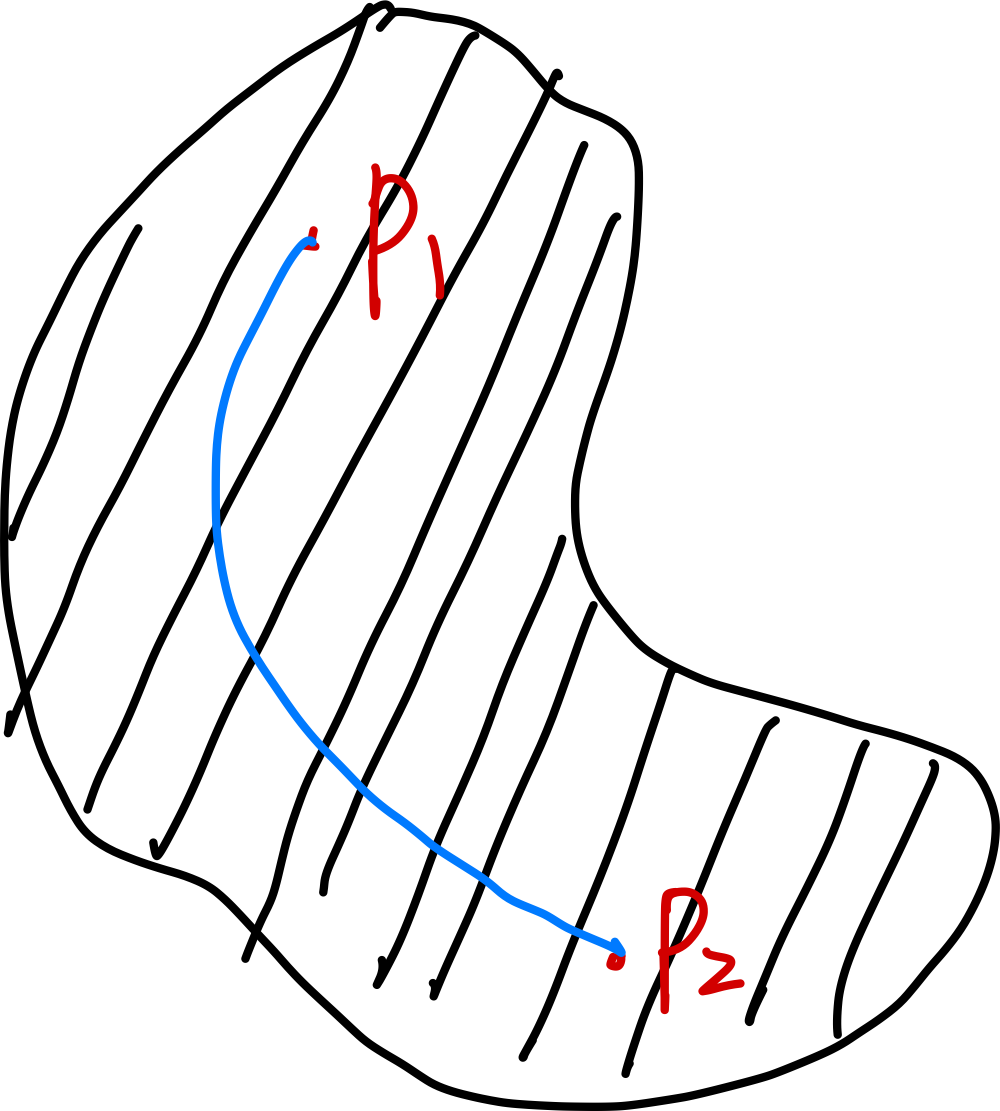
\includegraphics[scale=0.08]{"Chapter 08 images/pic1.png"}
        % \caption{}
        \label{pic1}
    \end{wrapfigure}

    要求过点\(M_{0}\left(2,1,3\right)\)且与直线$L$垂直相交的直线,关键在于求垂足\(M_1\)。
    可以作过点\(M_{0}\)且垂直于直线$L$的平面。

    则该平面的对称式方程为

    \[
        3(x-2)+2(y-1)-(z-3)=0
    \]

    即

    \[
        3x + 2y -z -5 =0
    \]

    \textbf{Part Two}

    再求直线与垂直平面的交点:

    令$\dfrac{x+1}{3}=\dfrac{y-1}{2}=\dfrac{z}{1}=t$

    得

    $$
        \left\{\begin{array}{l}
        x=-1+3 t \\
        y=1+2 t \\
        z=-t
        \end{array}\right.
    $$

    解得\(t=\dfrac{3}{7}\)

    代入得交点坐标为$\left(\dfrac{2}{7}, \dfrac{13}{7},-\dfrac{3}{7}\right)$

    \textbf{Part Three}

    所以所求直线的一个方向向量为

    $$
        \left(\frac{2}{7}-2, \frac{13}{7}-1,-\frac{3}{7}-3\right)=-\frac{6}{7}(2,-1,4)
    $$

    所以所求的直线方程为

    $$
        \frac{x-2}{2}=\frac{y-1}{-1}=\frac{z-3}{4}
    $$

\subsubsection{Problem 3}

    求直线$\left\{\begin{array}{l}x+y-z-1=0 \\ x-y+z+1=0\end{array}\right.$在平面\(x+y+z=0\)上投影
    直线的方程。
    \\

    \textbf{Solution}
    \\

    \begin{wrapfigure}{r}{4cm}
        \centering
        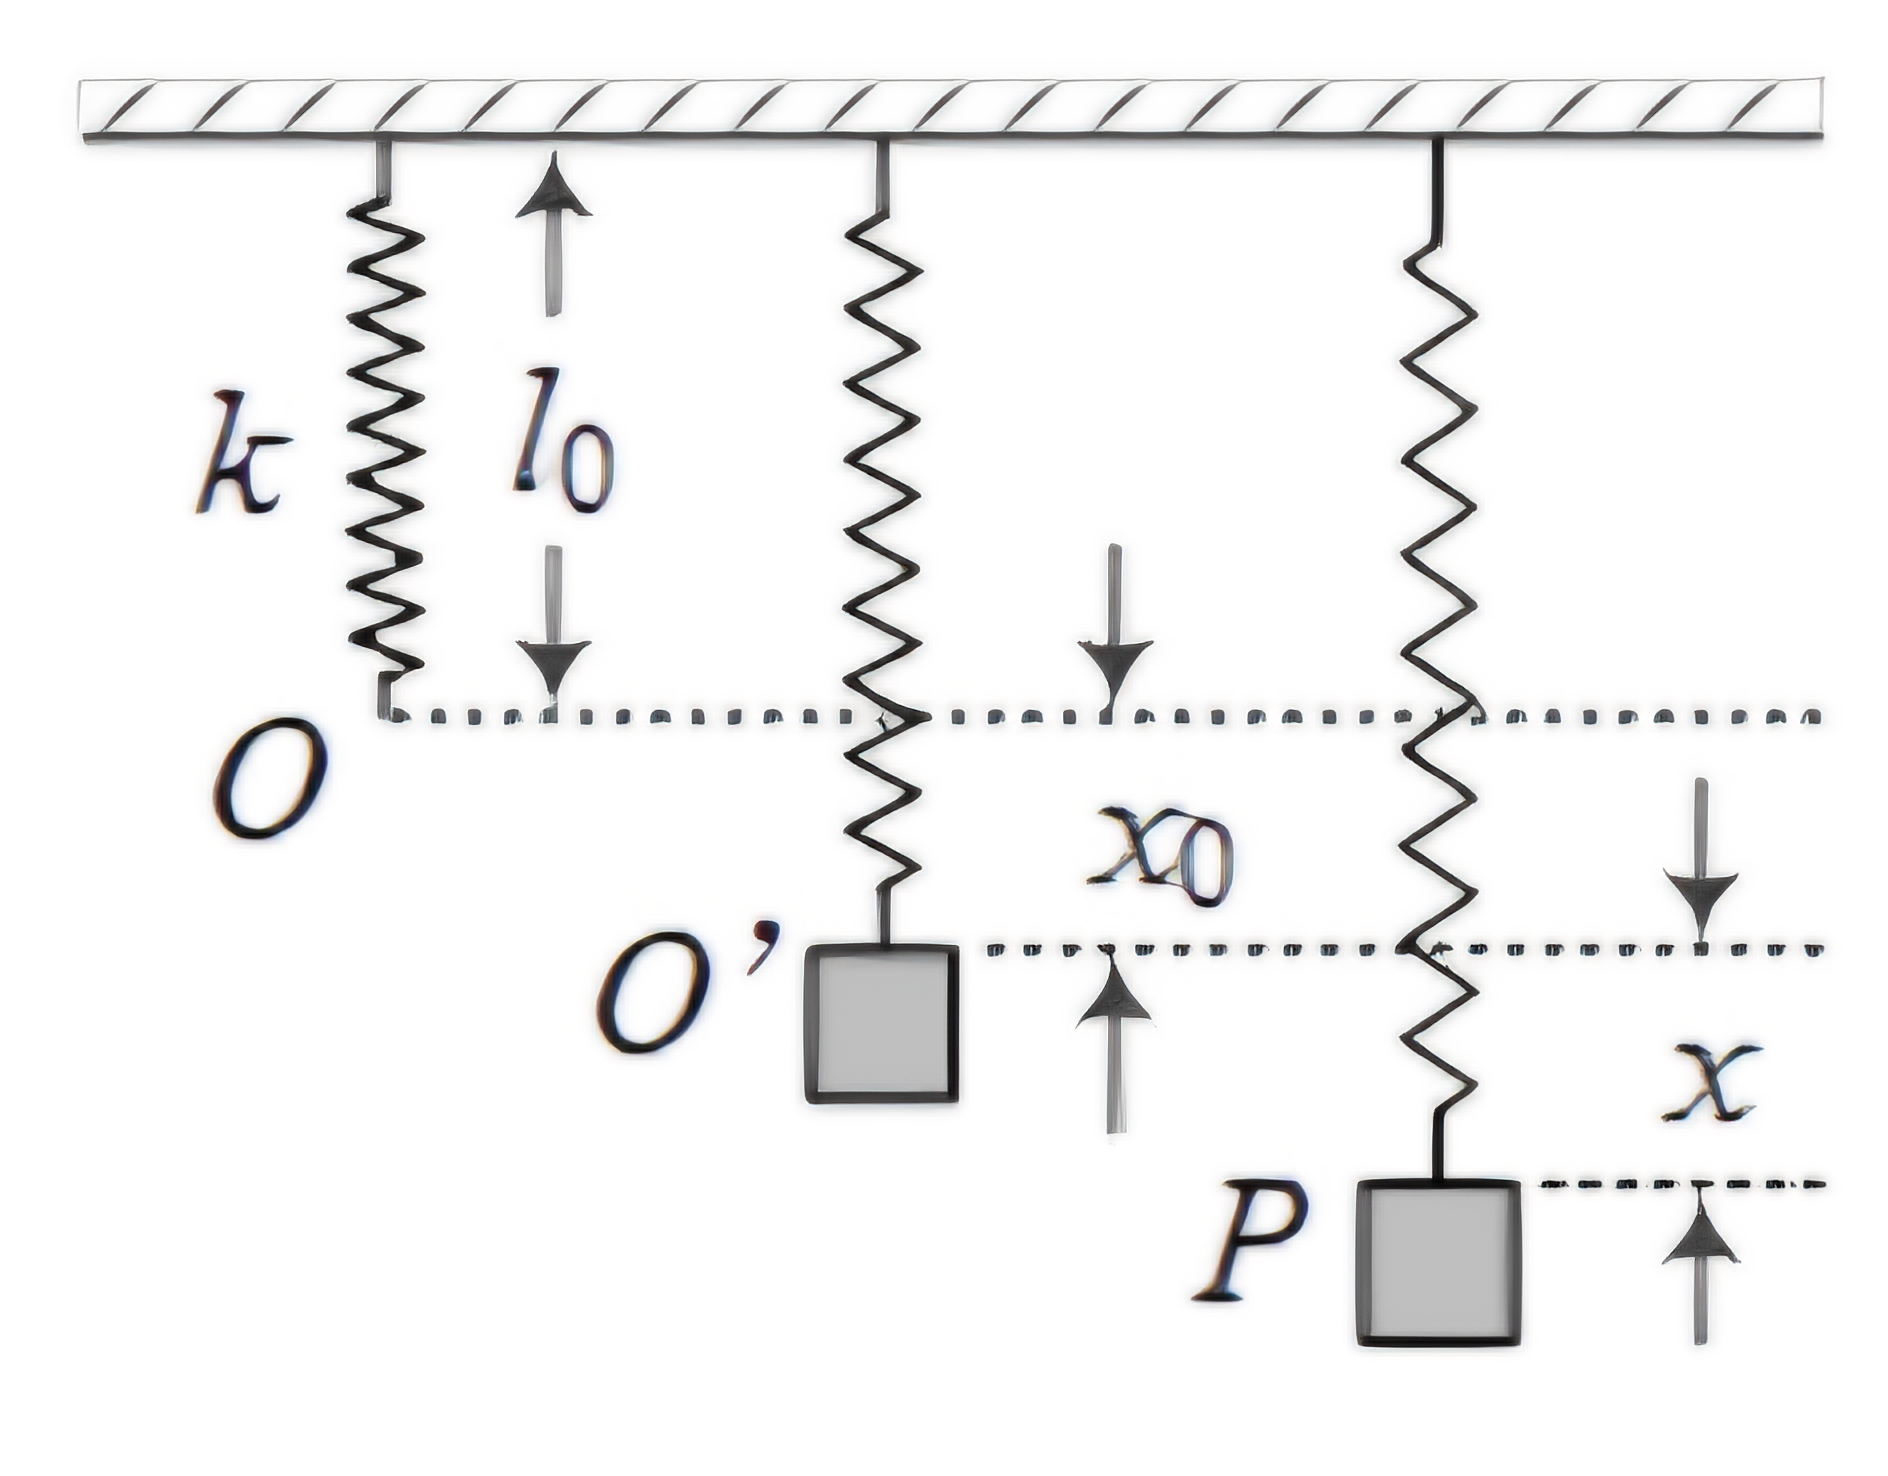
\includegraphics[scale=0.08]{"Chapter 08 images/pic2.png"}
        % \caption{}
        \label{pic2}
    \end{wrapfigure}

    过直线$\left\{\begin{array}{l}x+y-z-1=0 \\ x-y+z+1=0\end{array}\right.$的平面束方程为

    $$
        (x+y-z-1)+\lambda(x-y+z+1)=0
    $$

    整理得

    $$
        (1+\lambda) x+(1-\lambda) y+(-1+\lambda) z+(-1+\lambda)=0
    $$

    由于此平面与平面\(x+y+z=0\)垂直,则两平面法向量也相互垂直。即

    $$
        (1+\lambda) \cdot 1+(1-\lambda) \cdot 1+(-1+\lambda) \cdot 1=0
    $$

    解得\(\lambda=-1\)。

    代入平面束方程中,知投影直线的方程为

    $$
        \left\{\begin{array}{l}
        y-z-1=0 \\
        x+y+z=0
        \end{array}\right.
    $$

\section{曲面及其方程}

\subsection{曲面研究的基本问题}

\subsubsection{曲面的方程}

    若曲面\(S\)和三元方程\(F\left(x,y,z\right) = 0\)满足:

    \begin{enumerate}
        \item \(S\)上的点皆满足三元方程;
        \item 不在\(S\)上的点皆不满足三元方程;
    \end{enumerate}

    则称\(F\left(x,y,z\right) = 0\)为\(S\)的方程,\(S\)称为方程\(F\left(x,y,z\right) = 0\)的图形。

\subsubsection{两类基本问题}

    \begin{enumerate}
        \item 已知一曲面作为点的几何轨迹时,建立这曲面的方程;
        \item 已知坐标\(x\)、\(y\)和\(z\)间的一个方程时,研究这方程所表示的曲面的形状。
    \end{enumerate}

    \textbf{要求}:掌握常见的曲面及其方程。

    球心在点\(M_{0}\left(x_0,y_0,z_0\right)\)、半径为\(R\)的球面的方程为

    \begin{align}
        \left(x-x_0\right)^2+\left(y-y_0\right)^2+\left(z-z_0\right)^2=R^2
        \label{sphere-equation}
    \end{align}

    一般地,设有三元一次方程

    \[
        A x^2+A y^2+A z^2+D x+E y+F z+G=0
    \]

    方程中缺少\(x y, y z, z x\)各项,且平方项系数相同,只要经过配方可以化成方程\ref{sphere-equation}的形式,
    则它的图形就是一个球面。

\subsection{旋转曲面}

\subsubsection{定义}

    以一条平面曲线绕其平面上的一条直线旋转一周所成的曲面叫做旋转曲面,
    旋转曲线和定直线依次叫做旋转曲面的母线和轴。

    例如:

    \begin{figure}[htbp]
        \centering
        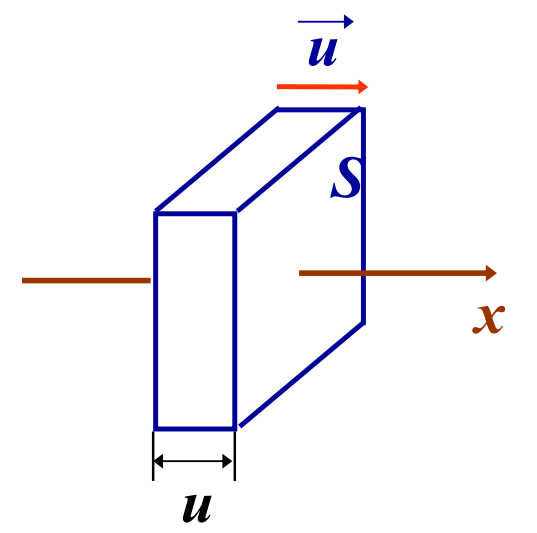
\includegraphics[scale=0.08]{"Chapter 08 images/pic3.png"}
    \end{figure}

    其中,\(C\)为旋转曲面的母线,\(L\)为旋转曲面的轴。

    \begin{figure}[htbp]
        \centering
        \subfigure[]
        {
            \begin{minipage}[b]{.3\linewidth}
                \centering
                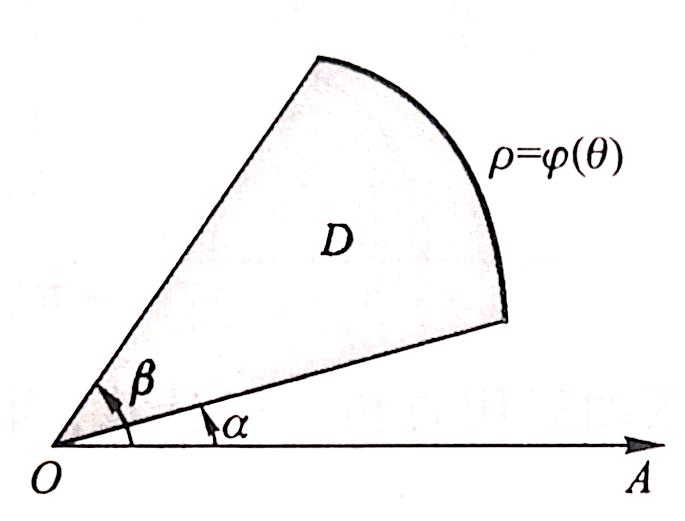
\includegraphics[scale=0.08]{"Chapter 08 images/pic4.png"}
            \end{minipage}
        }
        \subfigure[]
        {
             \begin{minipage}[b]{.3\linewidth}
                \centering
                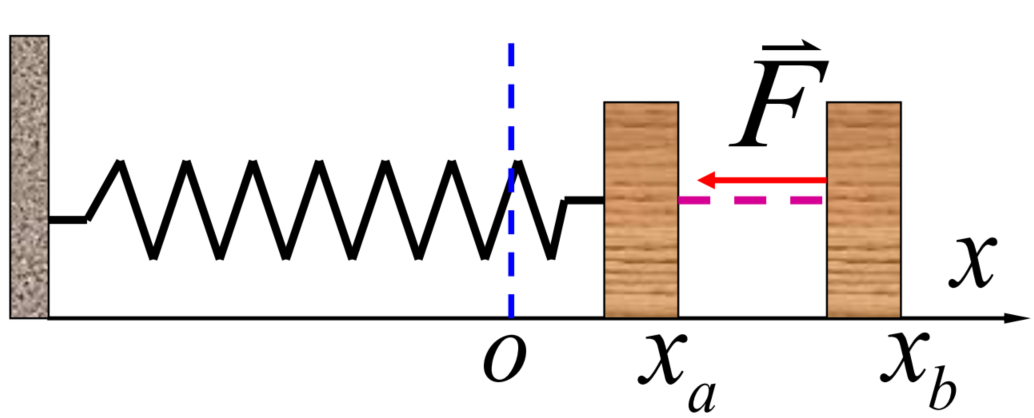
\includegraphics[scale=0.08]{"Chapter 08 images/pic5.png"}
            \end{minipage}
        }
        \subfigure[]
        {
             \begin{minipage}[b]{.3\linewidth}
                \centering
                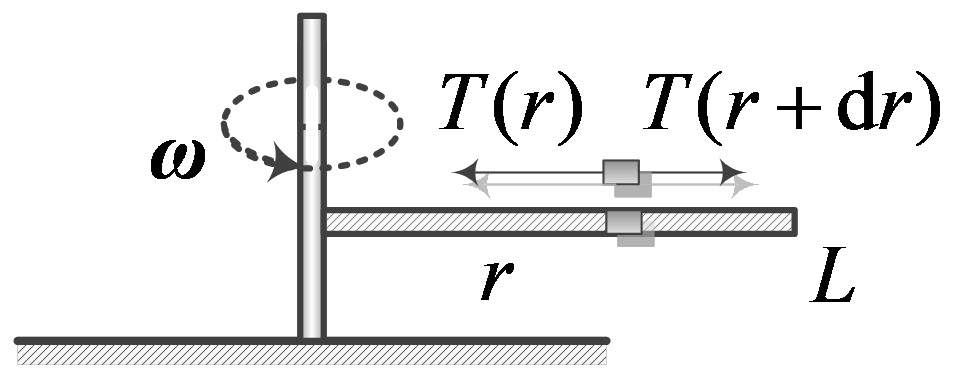
\includegraphics[scale=0.08]{"Chapter 08 images/pic6.png"}
            \end{minipage}
        }
    \end{figure}

    则图(a)中母线:\(z = a y^2\),轴:\(z\)轴;图(b)中母线:\(z = b y\),轴:\(z\)轴;
    图(c)中母线:\(y^2 + z^2 = R^2\),轴:\(z\)轴。
        
\subsubsection{旋转曲面的方程}

    \begin{wrapfigure}{r}{4cm}
        \centering
        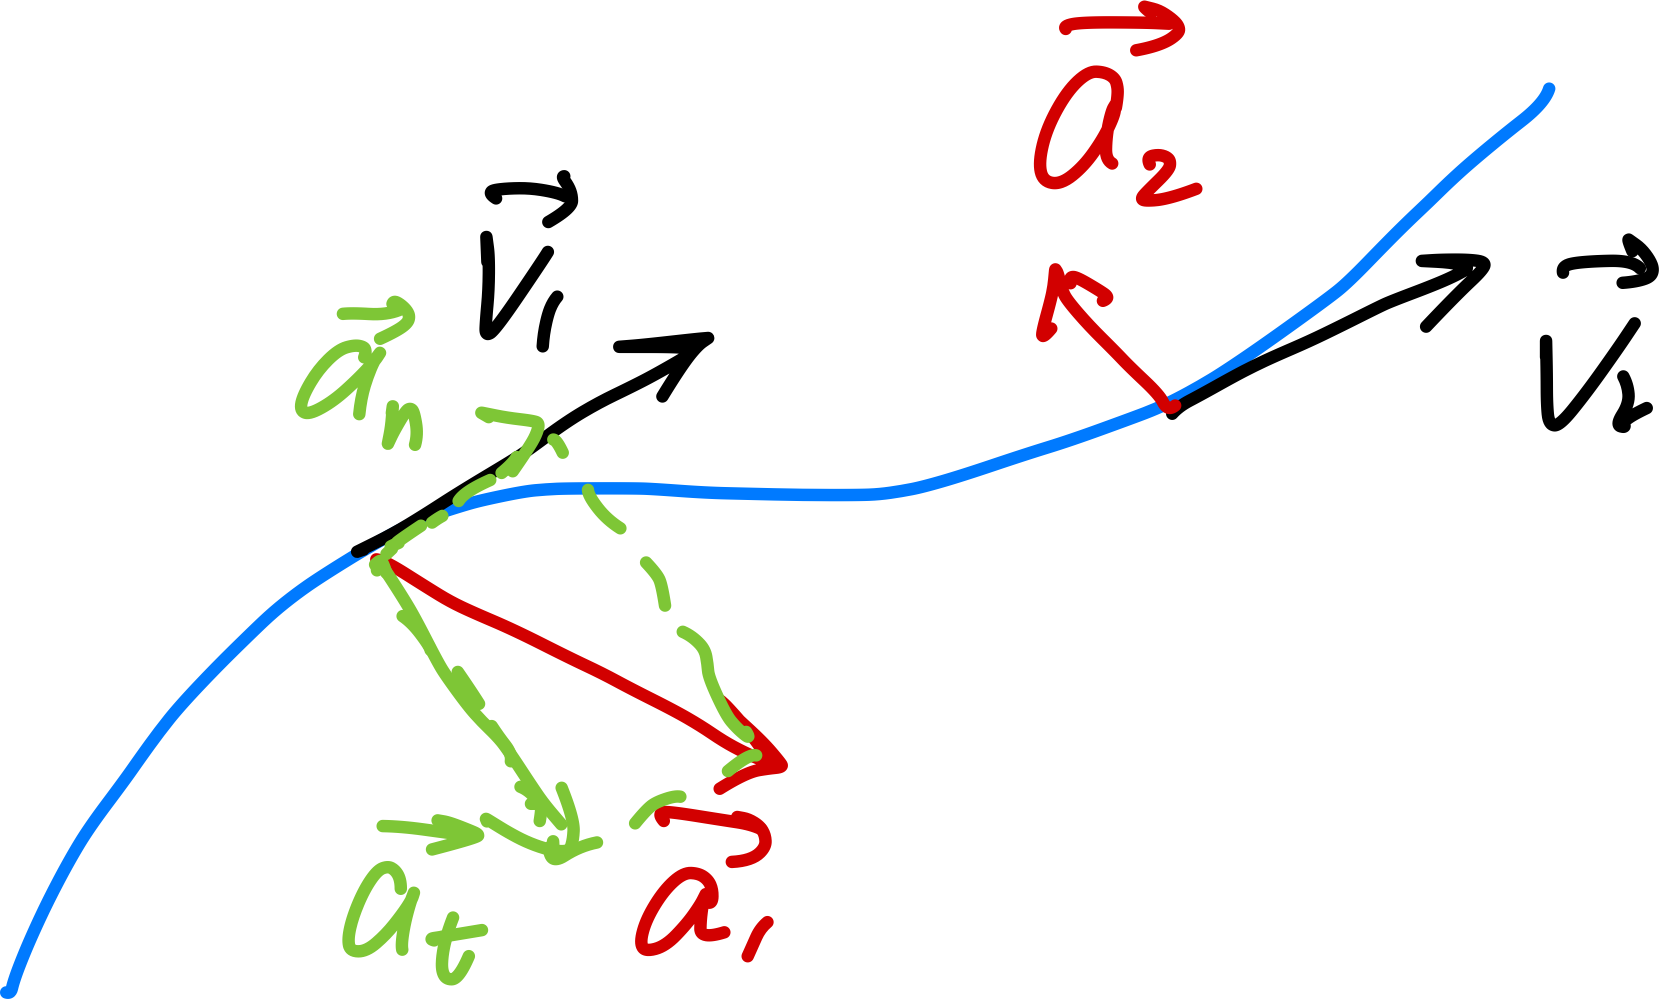
\includegraphics[scale=0.1]{"Chapter 08 images/pic7.png"}
        % \caption{}
        \label{pic7}
    \end{wrapfigure}

    设在\(yOz\)平面坐标面上有一已知曲线\(C: f\left(y,z\right) = 0\),则其以\(z\)轴为轴的旋转曲面的方程如下

    \begin{align}
        S: f\left(\pm \sqrt{x^2 + y^2},\; z\right) = 0
    \end{align}

    \textbf{推导:}

    \(\forall M\left(x,y,z\right) \in S\),设其由\(M_1 \in C\)转到某位置而得到。
    设\(M\left(x_1,y_1,z_1\right)\),则

    \begin{align}
        f\left(y_1, z_1\right) = 0
        \label{rotational-surface-2}
    \end{align}

    又\(M\)、\(M_1\)满足

    \begin{align*}
        \left\{\begin{aligned}
        z_1 & =z \cdot \\
        \left|y_1\right| & =\sqrt{x^2+y^2} \Rightarrow y_1= \pm \sqrt{x^2+y^2}
        \end{aligned}\right.
    \end{align*}

    代入式,得

    \begin{align*}
        f\left(\pm \sqrt{x^2 + y^2},\; z\right) = 0
    \end{align*}

    即为\(S\)上任一点\(M\left(x,y,z\right)\)满足的方程。

    总之,母线\(f\left(y, z\right) = 0\)

    \begin{align*}
        \left\{\begin{aligned}
        \text{绕\(z\)轴旋转}\rightarrow & S: f\left(\pm \sqrt{x^2 + y^2},\; z\right) = 0 \\
        \text{绕\(y\)轴旋转}\rightarrow & S: f\left(y,\; \pm \sqrt{z^2 + x^2}\right) = 0
        \end{aligned}\right.
    \end{align*}

    若母线\(f\left(z, x\right) = 0\)

    \begin{align*}
        \left\{\begin{aligned}
        \text{绕\(z\)轴旋转}\rightarrow & S: f\left(z,\; \pm \sqrt{x^2 + y^2}\right) = 0 \\
        \text{绕\(x\)轴旋转}\rightarrow & S: f\left(\pm \sqrt{y^2 + z^2},\; x\right) = 0
        \end{aligned}\right.
    \end{align*}

    若母线\(f\left(x, y\right) = 0\)

    \begin{align*}
        \left\{\begin{aligned}
        \text{绕\(x\)轴旋转}\rightarrow & S: f\left(x,\; \pm \sqrt{y^2 + z^2}\right) = 0 \\
        \text{绕\(y\)轴旋转}\rightarrow & S: f\left(\pm \sqrt{x^2 + z^2},\; y\right) = 0
        \end{aligned}\right.
    \end{align*}

\subsubsection{圆锥面}

    \begin{figure}[!h]
        \centering
        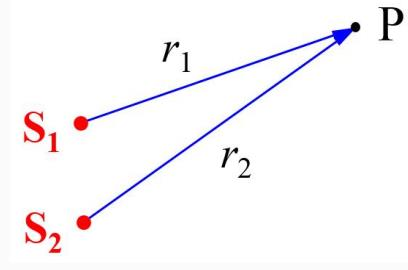
\includegraphics[scale=0.15]{"Chapter 08 images/pic8.png"}
        % \caption{}
        \label{pic8}
    \end{figure}

    直线\(L\)与另一条与\(L\)相交的直线旋转一周,所得曲面叫做圆锥面。两直线的交点称为顶点,
    两直线的夹角\(\alpha \; \left(0 < \alpha \dfrac{\mathrm{\pi}}{2}\right)\)叫做圆锥面的
    半顶角。

    则顶点在原点,轴为\(z\)轴,则半顶角为\(\alpha\)的圆锥面的方程为

    \begin{align}
        z^2 = \cot^2 \alpha \left(x^2 + y^2\right)
    \end{align}

    令\(a = \cot \alpha\)则圆锥面的方程为

    \begin{align}
        z^2 = a^2 \left(x^2 + y^2\right)
    \end{align}

    当\(a > 0\)时,有\(z = a \sqrt{x^2 + y^2}\)(上半锥面),\(z = -a \sqrt{x^2 + y^2}\)(下半锥面)。

    \textbf{常见锥面}

    \begin{enumerate}
        \item \(z = \sqrt{x^2 + y^2}\)(\(a = 1\)):半顶角为\(\alpha = \dfrac{\mathrm{\pi}}{4}\)上半锥面;
        \item \(z = -\sqrt{x^2 + y^2}\)(\(a = 1\)):半顶角为\(\alpha = \dfrac{\mathrm{\pi}}{4}\)下半锥面;
        \item \(z = \sqrt{3\left(x^2 + y^2\right)}\)(\(a = \sqrt{3}\)):半顶角为\(\alpha = \dfrac{\mathrm{\pi}}{6}\)上半锥面;
        \item \(z = 1- \sqrt{x^2 + y^2}\)(\(a = \sqrt{3}\)):顶点为\(\left(0,1\right)\)、开口向下、
            半顶角为\(\alpha = \dfrac{\mathrm{\pi}}{4}\)的上半锥面;
        \item \(z = \sqrt{x^2 + z^2}\)(\(a = \sqrt{3}\)):半顶角为\(\alpha = \dfrac{\mathrm{\pi}}{4}\),以\(y\)轴
            为轴的锥面。
    \end{enumerate}

\subsubsection{旋转抛物面}

    \(yOz\)平面上曲线\(z = a y^2\; \left(a > 0\right)\)绕\(z\)轴旋转一周而得的旋转体的方程为

    \begin{align}
        z_2 = a \left(x^2 + y^2\right)
    \end{align}

    该曲面称为旋转抛物面。

\subsubsection{旋转单叶/双叶双曲面}

    平面\(xOz\)平面上双曲线$\frac{x^2}{a^2}-\frac{z^2}{c^2}=1$

    绕\(z\)轴旋转一周,称为旋转单叶双曲面,其方程为:
    
    \begin{equation}
        \frac{x^2+y^2}{a^2}-\frac{z^2}{c^2}=1
    \end{equation}

    绕\(x\)轴旋转一周,称为旋转双叶双曲面,其方程为:

    \begin{equation}
        \frac{x^2}{a^2}-\frac{y^2+z^2}{c^2}=1
    \end{equation}

\subsection{柱面}

\subsubsection{分类讨论}

    \begin{enumerate}
        \item 一般地、只含\(x\)、\(y\)而缺\(z\)的方程\(F\left(x,y\right) =0\)在空间直角坐标系中表示母线
            平行于\(z\)轴的柱面,其准线是\(xOy\)面上的曲线\(C:F\left(x,y\right) =0\);
        \item 一般地、只含\(y\)、\(z\)而缺\(x\)的方程\(F\left(y,z\right) =0\)在空间直角坐标系中表示母线
            平行于\(x\)轴的柱面,其准线是\(xOy\)面上的曲线\(C:F\left(y,z\right) =0\);
        \item 一般地、只含\(z\)、\(x\)而缺\(y\)的方程\(F\left(z,x\right) =0\)在空间直角坐标系中表示母线
            平行于\(y\)轴的柱面,其准线是\(xOy\)面上的曲线\(C:F\left(z,x\right) =0\);
    \end{enumerate}
    
\subsection{二次曲面}

    与平面解析几何中规定的二次曲线相类似,我们把三元二次方程\(F\left(x,y,z\right) =0\)
    所表示的曲面称为二次曲面,把平面称为一次曲面。

\subsubsection{研究曲面的两种方法}

    \textbf{截痕法}

    以平面\(z=t\)(或\(x=t\),\(y=t\))去截曲面\(S\)得截痕,研究截痕随\(t\)变化规律,从而
    了解曲面的形状。

    \textbf{伸缩变形法}

    若原曲线方程为\(C: F\left(x,y,z\right) = 0\),将其沿着\(z\)轴伸缩\(\lambda\)倍,得方程为

    \begin{align}
        S^{'}: F\left(x, y, \frac{z}{\lambda}\right) = 0
    \end{align}

\subsection{九种二次曲面}

% TikZ图像代码来自https://blog.csdn.net/Daniel_tanxz/article/details/129889345

\subsubsection{椭圆锥面\(\dfrac{x^2}{a^2}+\dfrac{y^2}{b^2}=z^2\)}

    圆锥面方程:

    \[
        z^2 = x^2 + y^2
    \]

    沿\(x\)轴伸缩\(a\)倍:

    $$
        z^2=\frac{x^2}{a^2}+y^2
    $$

    沿\(y\)轴伸缩\(b\)倍:

    \begin{align}
        z^2=\frac{x^2}{a^2}+\frac{y^2}{b^2}
    \end{align}

    用平面\(z=t\)去截曲面得截痕为椭圆

    % 圆锥面
    \begin{center}
        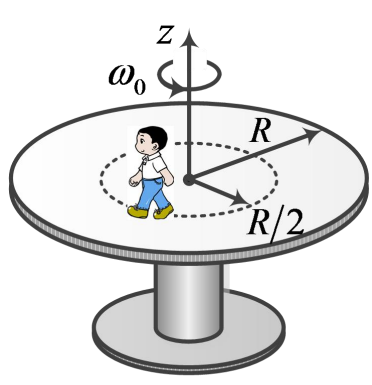
\includegraphics[height=6cm]{"Chapter 08 images/pic9.pdf"}
    \end{center}

\subsubsection{椭球面$\dfrac{x^2}{a^2}+\dfrac{y^2}{b^2}+\dfrac{z^2}{c^2}=1$}


    球面方程:

    \[
        x^2 + y^2 + z^2 = 1
    \]

    分别沿\(x\)、\(y\)、\(z\)轴伸缩\(a\)、\(b\)、\(c\)倍得

    \begin{equation}
        \frac{x^2}{a^2}+\frac{y^2}{b^2}+\frac{z^2}{c^2}=1
    \end{equation}

    % 椭球面
    \begin{center}
        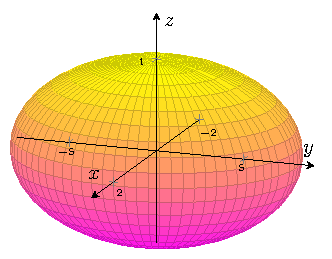
\includegraphics[height=6cm]{"Chapter 08 images/pic10.pdf"}
    \end{center}
    
\subsubsection{单叶双曲面$\dfrac{x^2}{a^2}+\dfrac{y^2}{b^2}-\dfrac{z^2}{c^2}=1$}

    旋转单叶双曲面方程:

    $$
        \frac{x^2}{a^2}+\frac{y^2}{a^2}-\frac{z^2}{c^2}=1
    $$

    沿\(y\)轴伸缩\(\frac{b}{a}\)倍:

    $$
        \frac{x^2}{a^2}+\frac{\left(\frac{a}{b} y\right)^2}{a^2}-\frac{z^2}{c^2}=1
    $$

    即:

    \begin{align}
        \dfrac{x^2}{a^2}+\dfrac{y^2}{b^2}-\dfrac{z^2}{c^2}=1
    \end{align}

    % 单叶双曲面
    \begin{center}
        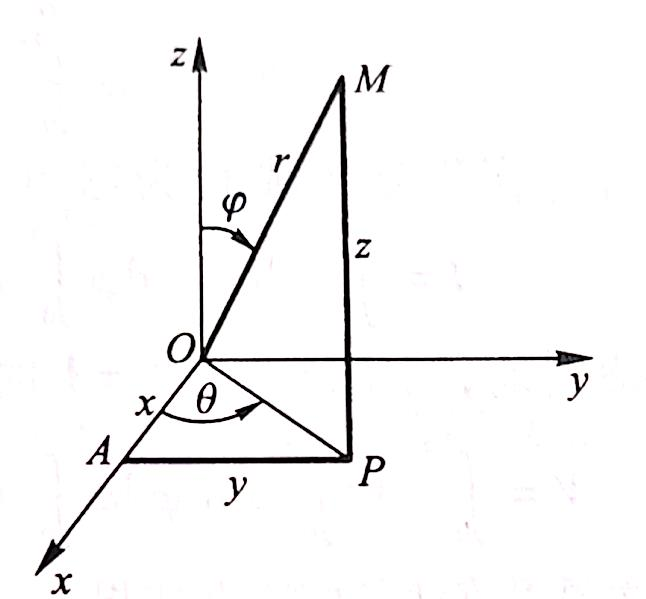
\includegraphics[height=6cm]{"Chapter 08 images/pic11.pdf"}
    \end{center}
  
\subsubsection{双叶双曲面$\dfrac{x^2}{a^2}-\dfrac{y^2}{b^2}-\dfrac{z^2}{c^2}=1$}
    旋转单叶双曲面方程:

    $$
        \frac{x^2}{a^2}-\frac{y^2}{b^2}-\frac{z^2}{b^2}=1
    $$

    沿\(z\)轴伸缩\(\frac{c}{b}\)倍:

    $$
        \frac{x^2}{a^2}-\frac{y^2}{b^2}-\frac{\left(\frac{b}{c} z\right)^2}{b^2}=1
    $$

    即:

    \begin{align}
        \dfrac{x^2}{a^2}-\dfrac{y^2}{b^2}-\dfrac{z^2}{c^2}=1
    \end{align}

    % 双叶双曲面
    \begin{center}
        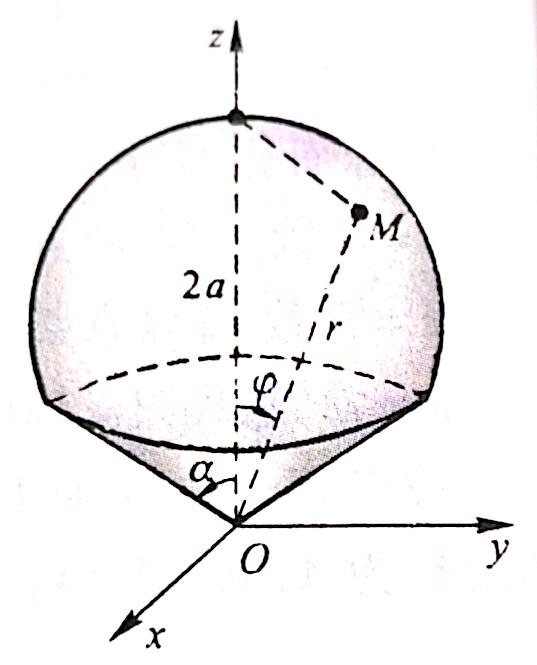
\includegraphics[height=6cm]{"Chapter 08 images/pic12.pdf"}
    \end{center}
    
\subsubsection{椭圆抛物面$\dfrac{x^2}{a^2}+\dfrac{y^2}{b^2}=z$}

    参考旋转抛物面方程:

    $$
        z=\frac{x^2+y^2}{a^2}
    $$

    伸缩可得

    \begin{equation}
        \frac{x^2}{a^2}+\frac{y^2}{b^2}=z
    \end{equation}

    % 椭圆抛物面
    \begin{center}
        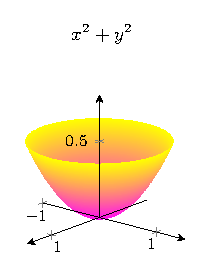
\includegraphics[height=6cm]{"Chapter 08 images/pic13.pdf"}
    \end{center}

\subsubsection{双曲抛物面$\dfrac{x^2}{a^2}-\dfrac{y^2}{b^2}=z$}
    
    % 双曲抛物面
    \begin{center}
        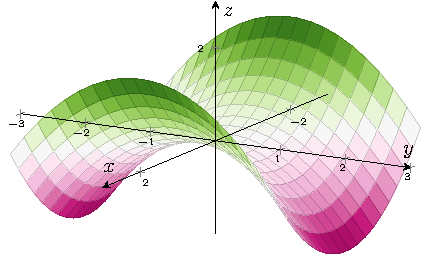
\includegraphics[height=6cm]{"Chapter 08 images/pic14.pdf"}
    \end{center}
    
\subsubsection{椭圆柱面$\dfrac{x^2}{a^2}+\dfrac{y^2}{b^2}=1$}

    % 椭圆柱面
    \begin{center}
        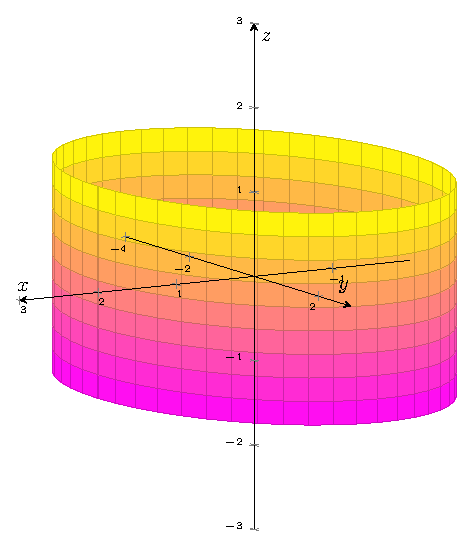
\includegraphics[height=6cm]{"Chapter 08 images/pic15.pdf"}
    \end{center}

\subsubsection{双曲柱面$\dfrac{x^2}{a^2}-\dfrac{y^2}{b^2}=1$}
    
    % 双曲柱面
    \begin{center}
        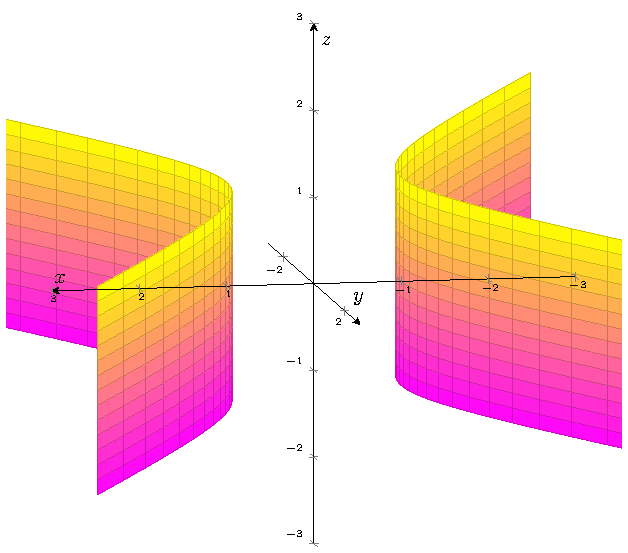
\includegraphics[height=6cm]{"Chapter 08 images/pic16.pdf"}
    \end{center}

\subsubsection{抛物柱面$x^2=ay$}

    % 抛物柱面
    \begin{center}
        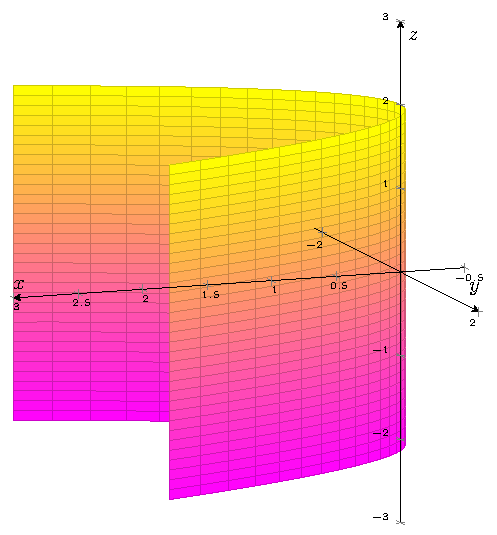
\includegraphics[height=6cm]{"Chapter 08 images/pic17.pdf"}
    \end{center}

\section{空间曲线及其方程}

\subsection{空间曲线的一般方程}

    \textbf{定义}

    设有空间曲线\(C\),以及过\(C\)的两张曲面\(S_1: F\left(x,y,z\right)\)和\(S_2: G\left(x,y,z\right)\),
    则称方程组

    \begin{equation}
        \left\{\begin{array}{l}
        F(x, y, z)=0 \\
        G(x, y, z)=0
        \end{array}\right.
    \end{equation}

    为空间曲线\(C\)的一般方程。

    注意:

    \begin{enumerate}
        \item \(C\)的一般方程不唯一;
        \item 平面曲线\(C: f\left(x,y\right)=0\)可以看作空间曲线,其一般方程为
            \begin{align*}
                \left\{\begin{array}{l}
                f(x, y)=0 \\
                z=0
                \end{array}\right.
            \end{align*}
    \end{enumerate}

\subsection{空间曲线的参数方程}

    \textbf{定义}

    若有方程

    \begin{equation}
        \left\{\begin{array}{l}
        x=\varphi\left(t\right) \\
        y=\phi\left(t\right) \\
        z=\omega\left(t\right)
        \end{array}\right.
        \label{Parametric equations of a space curve}
    \end{equation}

    其中\(t \in \left[\alpha, \beta\right]\),即空间曲线\(C\),若满足

    \begin{enumerate}
        \item \(\forall t \in \left[\alpha, \beta\right]\),点\(\left(
            \varphi\left(t\right),\phi\left(t\right),\omega\left(t\right)\right)\)
            在曲线\(C\)上;
        \item 对\(C\)上任意一点\(M\left(x,y,z\right)\),存在\(t_0 \in \left[\alpha, \beta\right]\),
            使得x\(=\varphi\left(t\right),\; y=\phi\left(t\right),\; z=\omega\left(t\right)\)。
    \end{enumerate}

    则称方程\ref{Parametric equations of a space curve}为空间曲线的参数方程。

    例如,空间曲线$\left\{\begin{array}{c}x+y-z=1 \\ z=x^2\end{array}\right.$
    的参数方程为$\left\{\begin{array}{l}x=t \\ y=1-t+t^2 \\ z=t^2\end{array}\right.$。

\subsection{空间曲线在坐标面上的投影}

    设有空间曲线$C: \left\{\begin{array}{l} F(x, y, z)=0 \\ G(x, y, z)=0 \end{array}\right.$,
    要求其在\(xOy\)面上的投影。

    注意到\(xOy\)面上的都不显含\(z\)。从方程组中消去变量\(z\)得

    \begin{align}
        H\left(x,y\right) = 0
        \label{H equals 0}
    \end{align}

    研究方程\ref{H equals 0}知:该方程表示母线平行与\(z\)轴的柱面,且该方程通过曲线\(C\)。
    于是\textbf{定义}曲面\ref{H equals 0}为曲线\(C\)关于\(xOy\)面的投影柱面。

    联立方程

    \begin{equation}
        \left\{\begin{array}{l}
        H\left(x,y\right) = 0 \\
        z=0
        \end{array}\right.
    \end{equation}

    即得到曲线\(C\)的投影曲线。

    同理,消去方程中的变量\(x\)或变量\(y\),再分别和\(x=0\)或\(y=0\)联立,即可得到曲线\(C\)
    在\(yOz\)面或\(xOz\)上的投影的曲线方程:

    \begin{equation}
        \left\{\begin{array}{l}
        R\left(y,z\right) = 0 \\
        x=0
        \end{array}\right.
    \end{equation}

    或

    \begin{equation}
        \left\{\begin{array}{l}
        T\left(x,z\right) = 0 \\
        y=0
        \end{array}\right.
    \end{equation}

\subsection{例题}

    设一个立体由上半球面\(z = \sqrt{4-x^2-y^2}\)和锥面\(z = \sqrt{6\left(x^2+y^2\right)}\)所围成
    (如下图所示),求它在\(xOy\)面上的投影。

    \begin{center}
        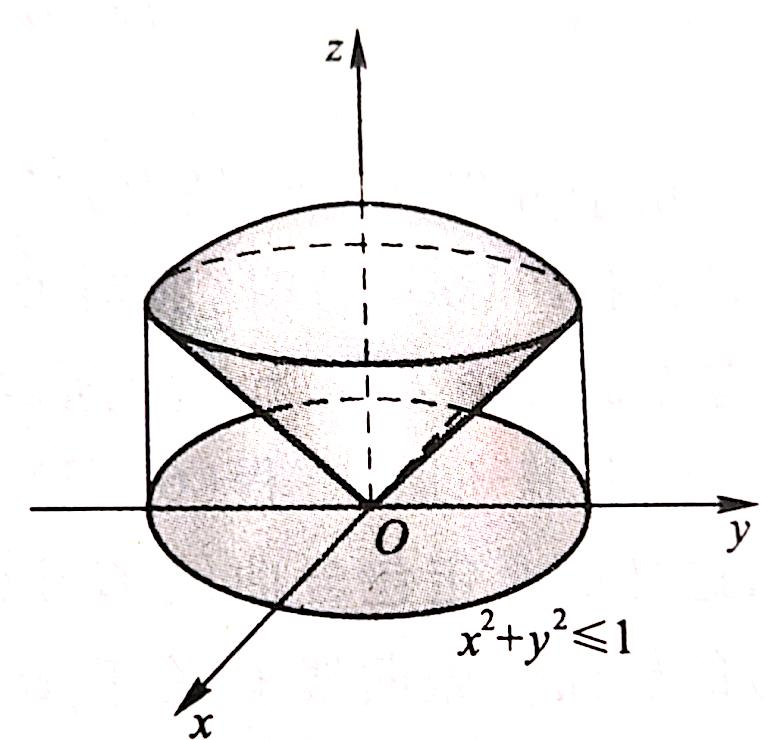
\includegraphics[height=3cm]{"Chapter 08 images/pic18.jpg"}
    \end{center}

    \textbf{Solution}
    \\

    两曲面交线为

    $$
        \left\{\begin{array}{l}
        z=\sqrt{4-x^2-y^2} \\
        z=\sqrt{3\left(x^2+y^2\right)}
        \end{array}\right.
    $$

    从中消去\(z\)得投影柱面\(x^2 + y^2 = 1\),将其与\(z=0\)联立,得投影曲线

    $$
        \left\{\begin{array}{l}
        x^2+y^2=1 \\
        z=0
        \end{array}\right.
    $$

    从而得投影区域为\(xOy\)面上的圆域

    $$
    D_{xy}: x^2 + y^2 \leq 1
    $$

\end{document}
